% ****************************************************************************************************
% Appendix: Additional Waterfall Plots
% ****************************************************************************************************

\chapter{Additional SHAP Waterfall Plots}
\label{app:waterfalls}

This appendix collects the SHAP waterfall plots not shown in the main body of Chapter~\ref{ch:explainability}. For each ESI class, three patients were selected: the highest-confidence correct prediction, the lowest-confidence correct prediction, and a misclassified case (with preference for under-triage). Chapter~\ref{ch:explainability} presents four of these pairs in detail; the remaining pair (ESI-3) is shown here.

\begin{figure}[htbp]
 \centering
 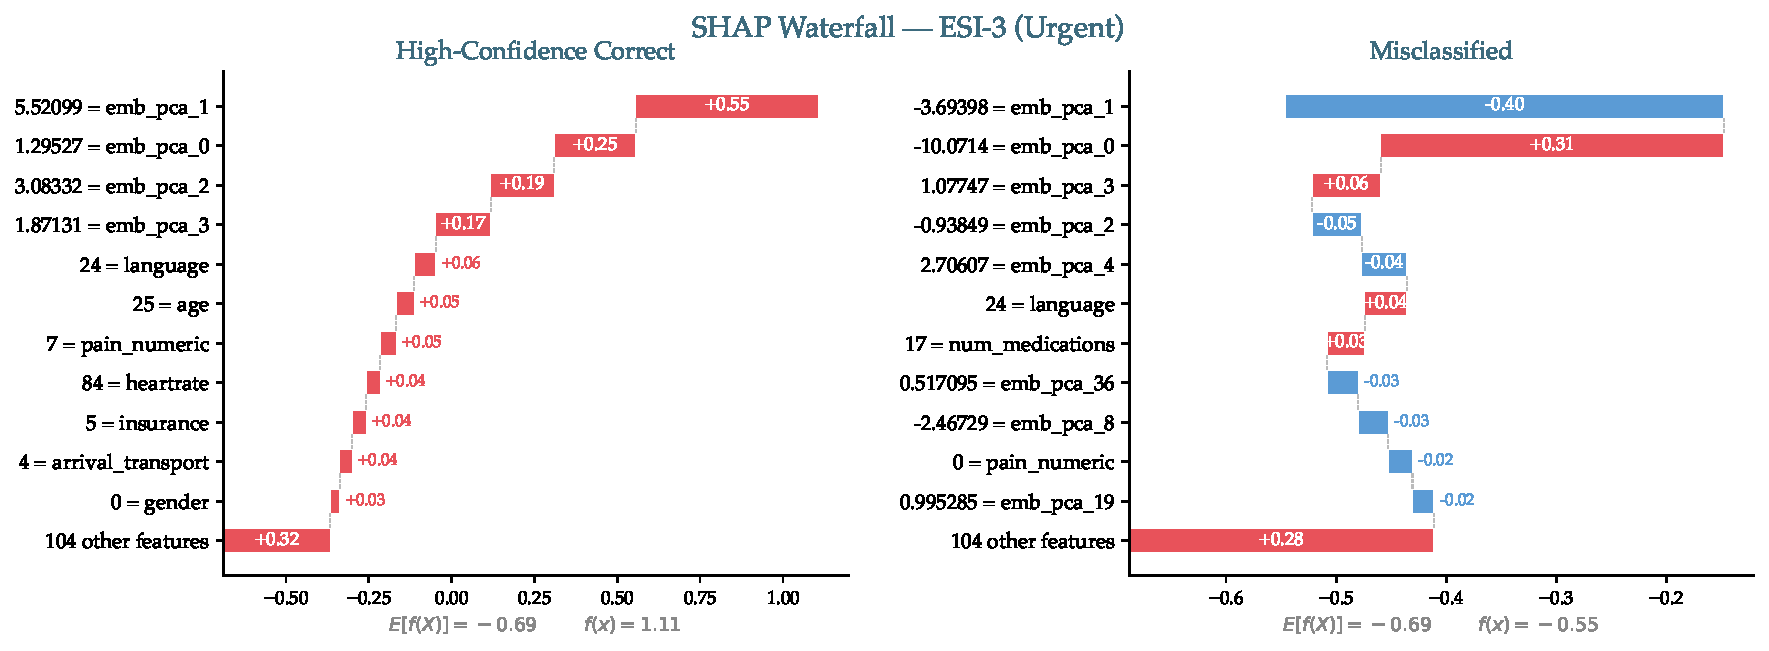
\includegraphics[width=\textwidth]{figures/shap_waterfall_esi3.pdf}
 \caption[Waterfall: ESI-3 (urgent)]{Waterfall plots for two ESI-3 patients. Left: high-confidence correct prediction. Right: misclassified (predicted ESI-4). The ESI-3 misclassification pattern typically involves moderate embedding signal with clinical features (heart rate, pain score) that are not alarming enough to push the prediction above the ESI-3/ESI-4 boundary.}
 \label{fig:waterfall-esi3}
\end{figure}
